\begin{newpage}
  \section{Problemlösungsprozess}
  \label{sec:problemlösungsprozess}
    Dieses Kapitel soll den durchlaufenen Prozess sowie die einzelnen Schritte beschreiben, die zur Realisierung des Projekts unternommen wurden. 

    Das Projekt wurde nach dem Design Prozess \texttt{"`The Double Diamond"'}\footnote{\url{http://www.designcouncil.org.uk/news-opinion/design-process-what-double-diamond}} bearbeitet. Der Double Diamond wurde vom British Design Council 2005 entwickelt und soll im folgenden danach beschrieben werden.\parencite{designcouncil}

    \begin{figure}[htbp]
      \begin{center}
        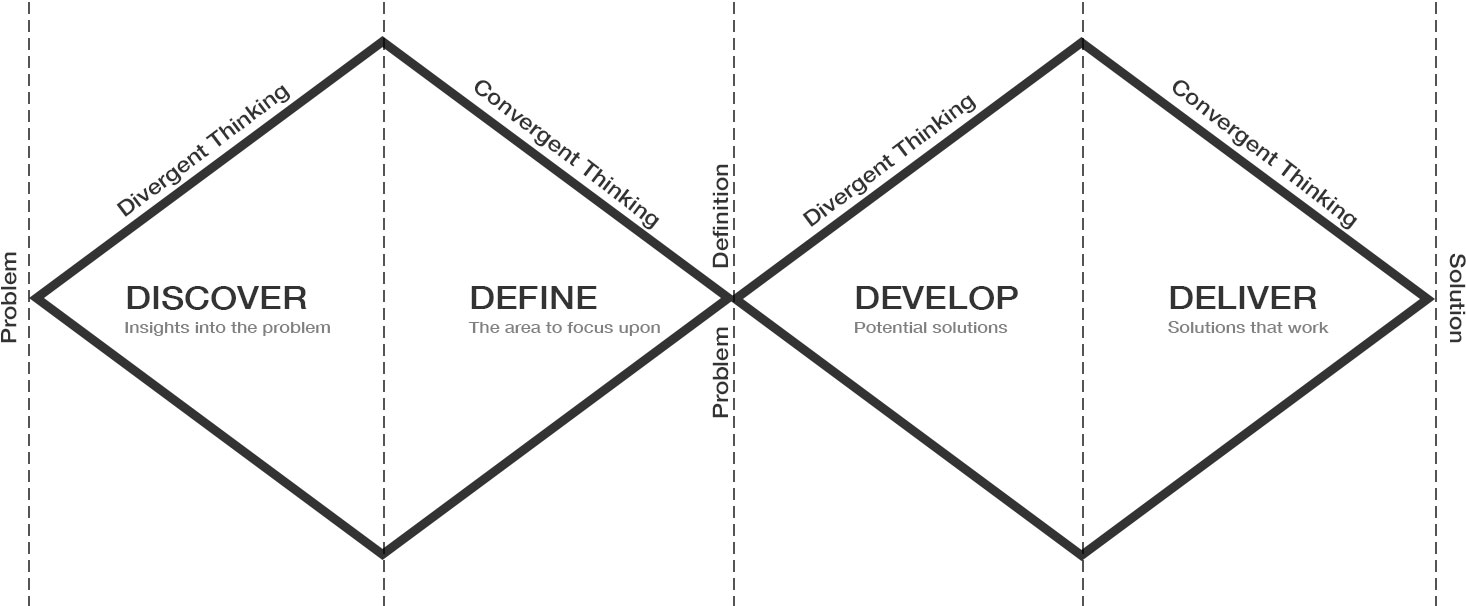
\includegraphics[width=0.9\textwidth]{double_diamond}
        \caption{"`The Double Diamond"' eigene Abbildung nach \parencite{designcouncil}}
        \label{fig:double_diamond}
      \end{center}
    \end{figure}

    Der Double Diamond beschreibt ein iterative Prozess. Wie in allen kreativen Prozessen werden dabei eine Reihe von möglichen Ideen geschaffen ("divergentes Denken"), bevor sie verfeinert und auf die beste Idee reduziert werden ("konvergentes Denken"). Der Double Diamond zeigt jedoch an, dass dies zweimal geschieht - einmal zur Bestätigung der Problemdefinition und einmal zur Erstellung der Lösung. Einer der größten Fehler ist es, den linken Diamanten wegzulassen und am Ende das falsche Problem zu lösen.

    \begin{itemize}[label={}]
      \item \textbf{Discover:} Der erste Teil des Double Diamond steht am Anfang des Projektes. Hier wird versucht, die Welt neu zu sehen, Neues wahrzunehmen und Einsichten in das zu lösende Problem zu sammeln.

      \item \textbf{Define:} Der zweite Teil stell die Definitionsphase dar. Dabei wird versucht alle in der Entdeckungsphase identifizierten Möglichkeiten zu verstehen. Ziel ist es dabei, ein klares Briefing zu entwickeln, das die grundsätzlichen Herausforderungen umrahmt.

      \item \textbf{Develop:} Der dritte Teil markiert eine Entwicklungsphase, in der Lösungen oder Konzepte erstellt, prototypisiert, getestet und iteriert werden. Dieser Prozess des Ausprobierens hilft, Ideen zu verbessern und zu verfeinern.

      \item \textbf{Deliver:} Der letzte Teil des Double Diamond ist die Lieferphase, in der das daraus resultierende Projekt (z. B. ein Produkt, eine Dienstleistung oder eine Umwelt) abgeschlossen, produziert und in Betrieb genommen wird.
    \end{itemize}
    

    \subsection{Discover}
    \label{sub:discover}
      Dafür erfolgte eine weitreichende Recherche zu relevanten Themenbereichen wie Live Visualisierung, Visualisierung von öffentlichem Nahverkehr sowie Tools zum Erstellen von Karten (Abbildung \ref{fig:viz_overview}). 

      \begin{figure}[ht]
        \begin{center}
          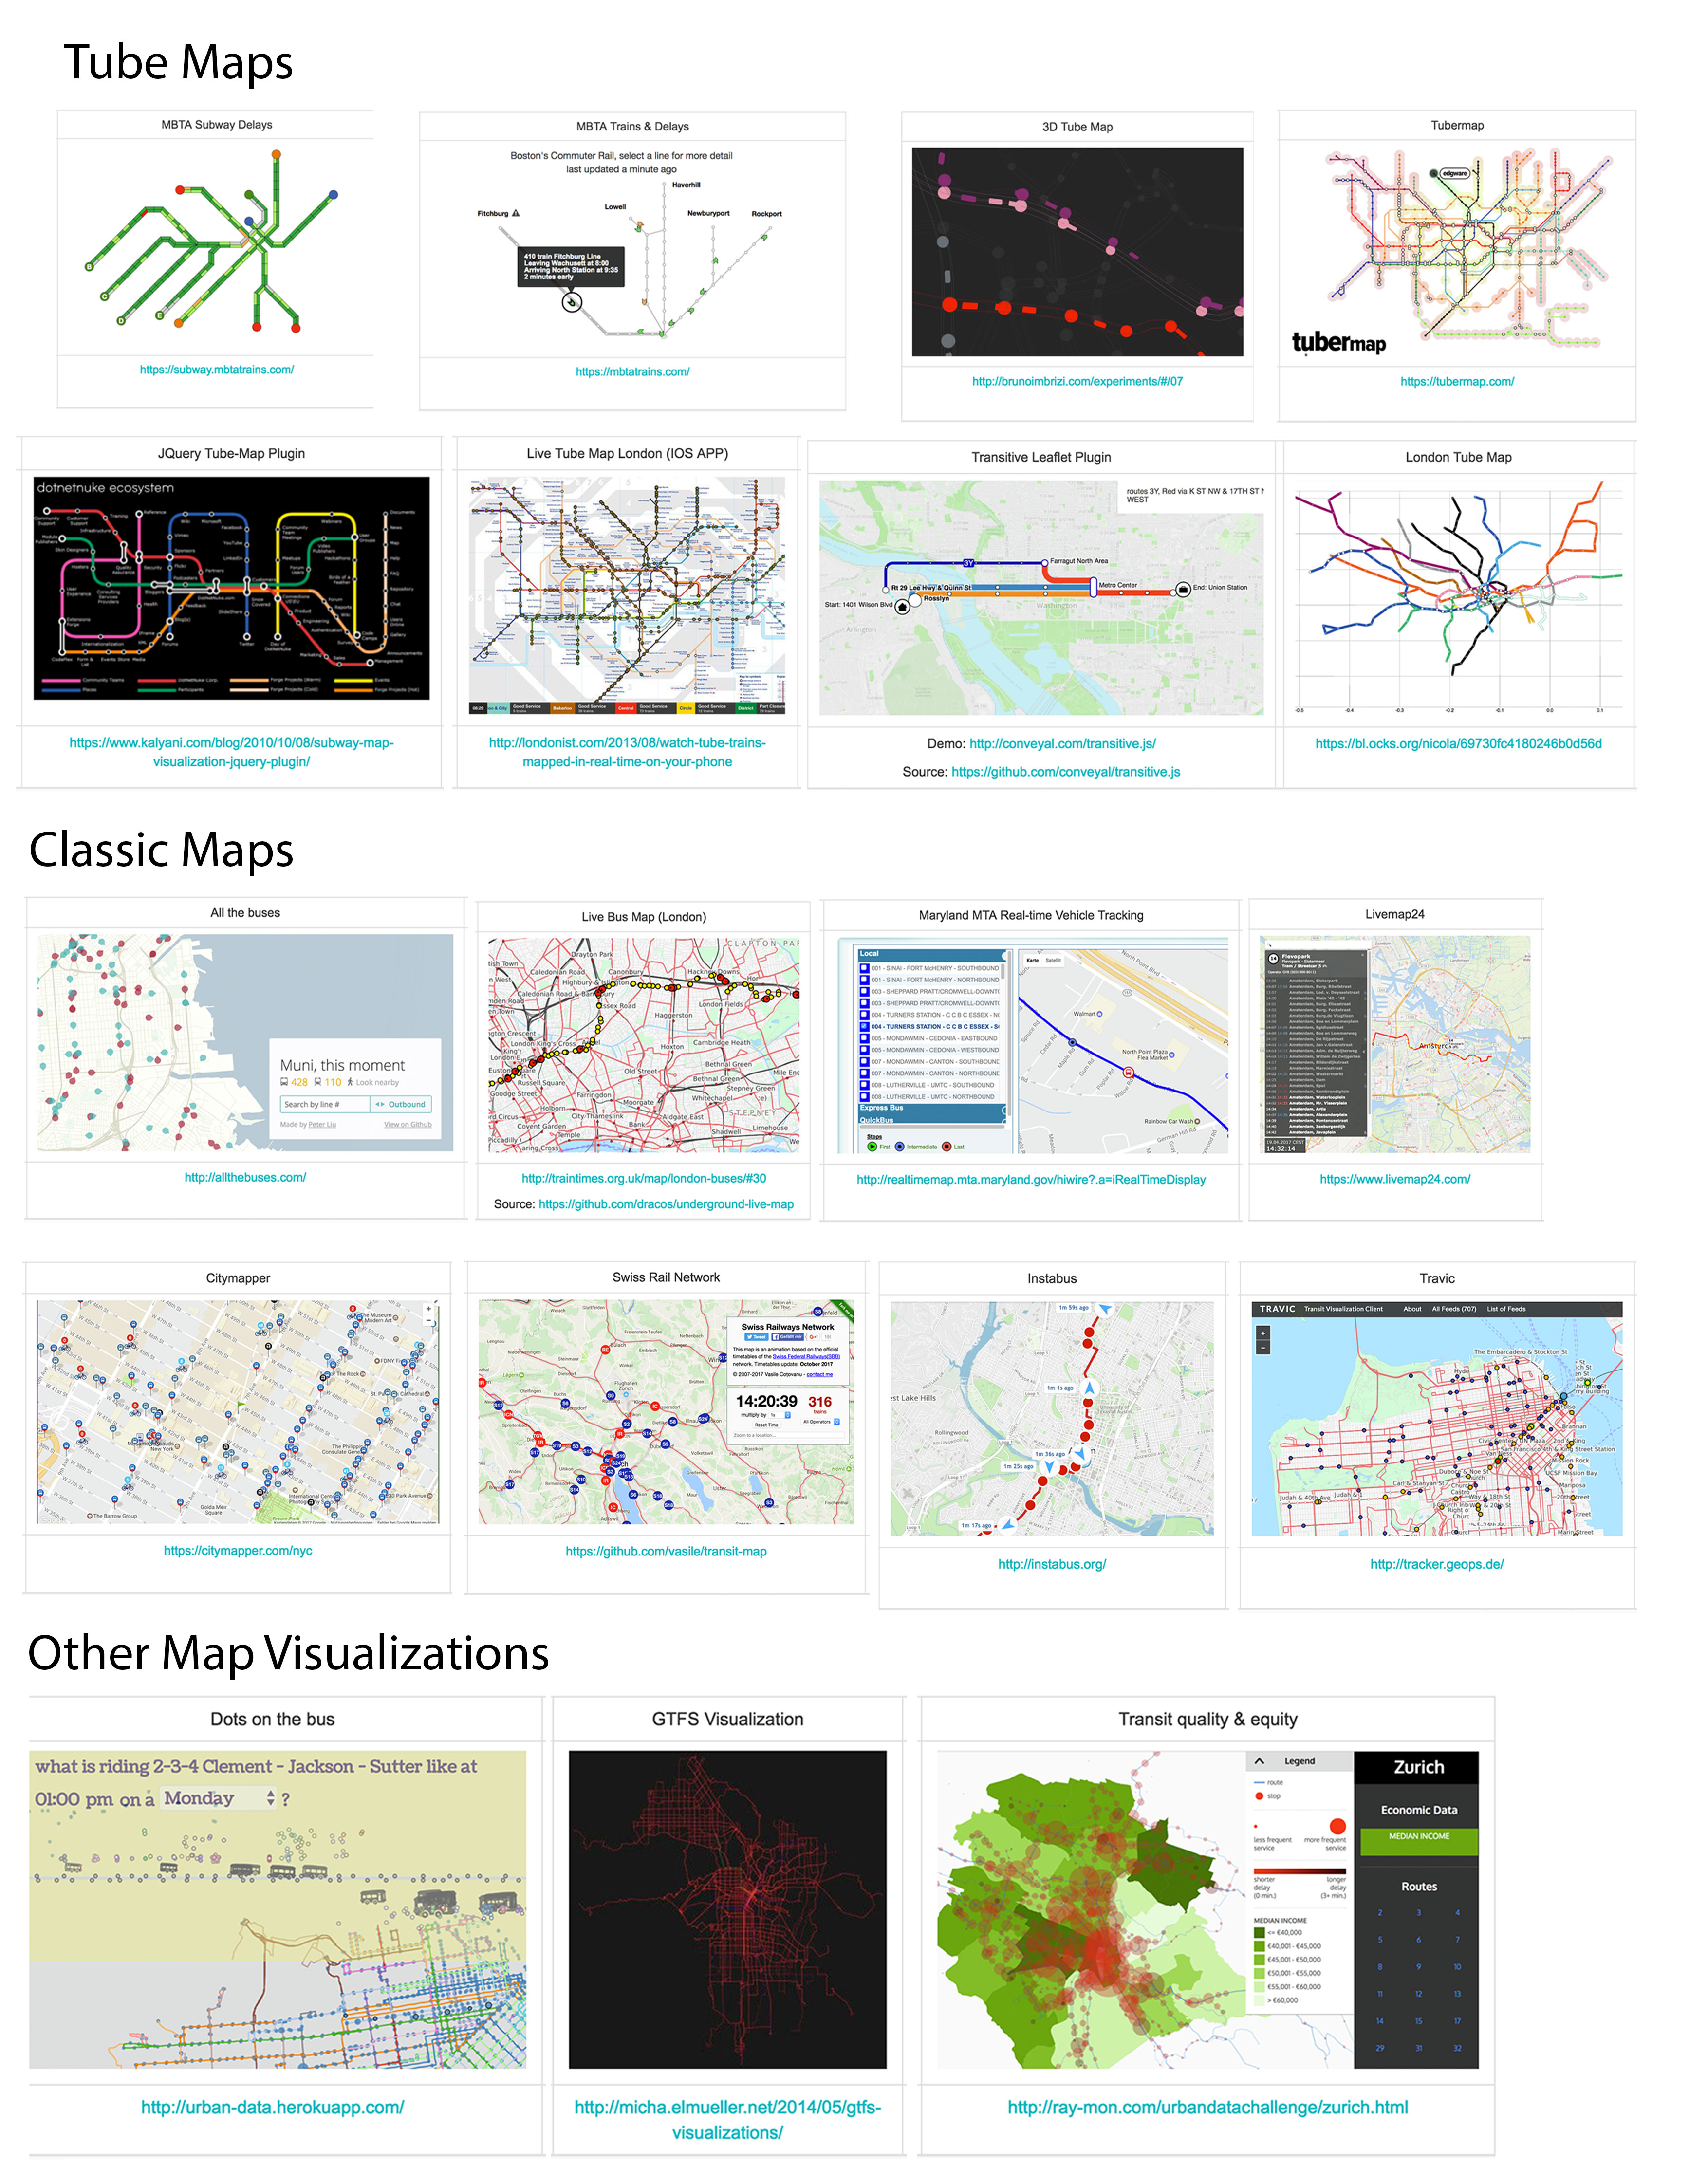
\includegraphics[width=0.80\textwidth]{viz_overview}
          \caption{Überblick über bestehende Tools und Visualisierungen}
          \label{fig:viz_overview}
        \end{center}
      \end{figure}

      Das gesammelte Material wurde in einer 2x2 Matrix (Abbildung \ref{fig:2x2_matrix}) in die Unterkategorien "`Live Map, Künstlerische Visualisierung, Plugin / Software / Tool, Tube-Map"' eingeordnet um einen sortierten Gesamtüberblick zu bekommen. 

      \begin{figure}[htbp]
        \begin{center}
          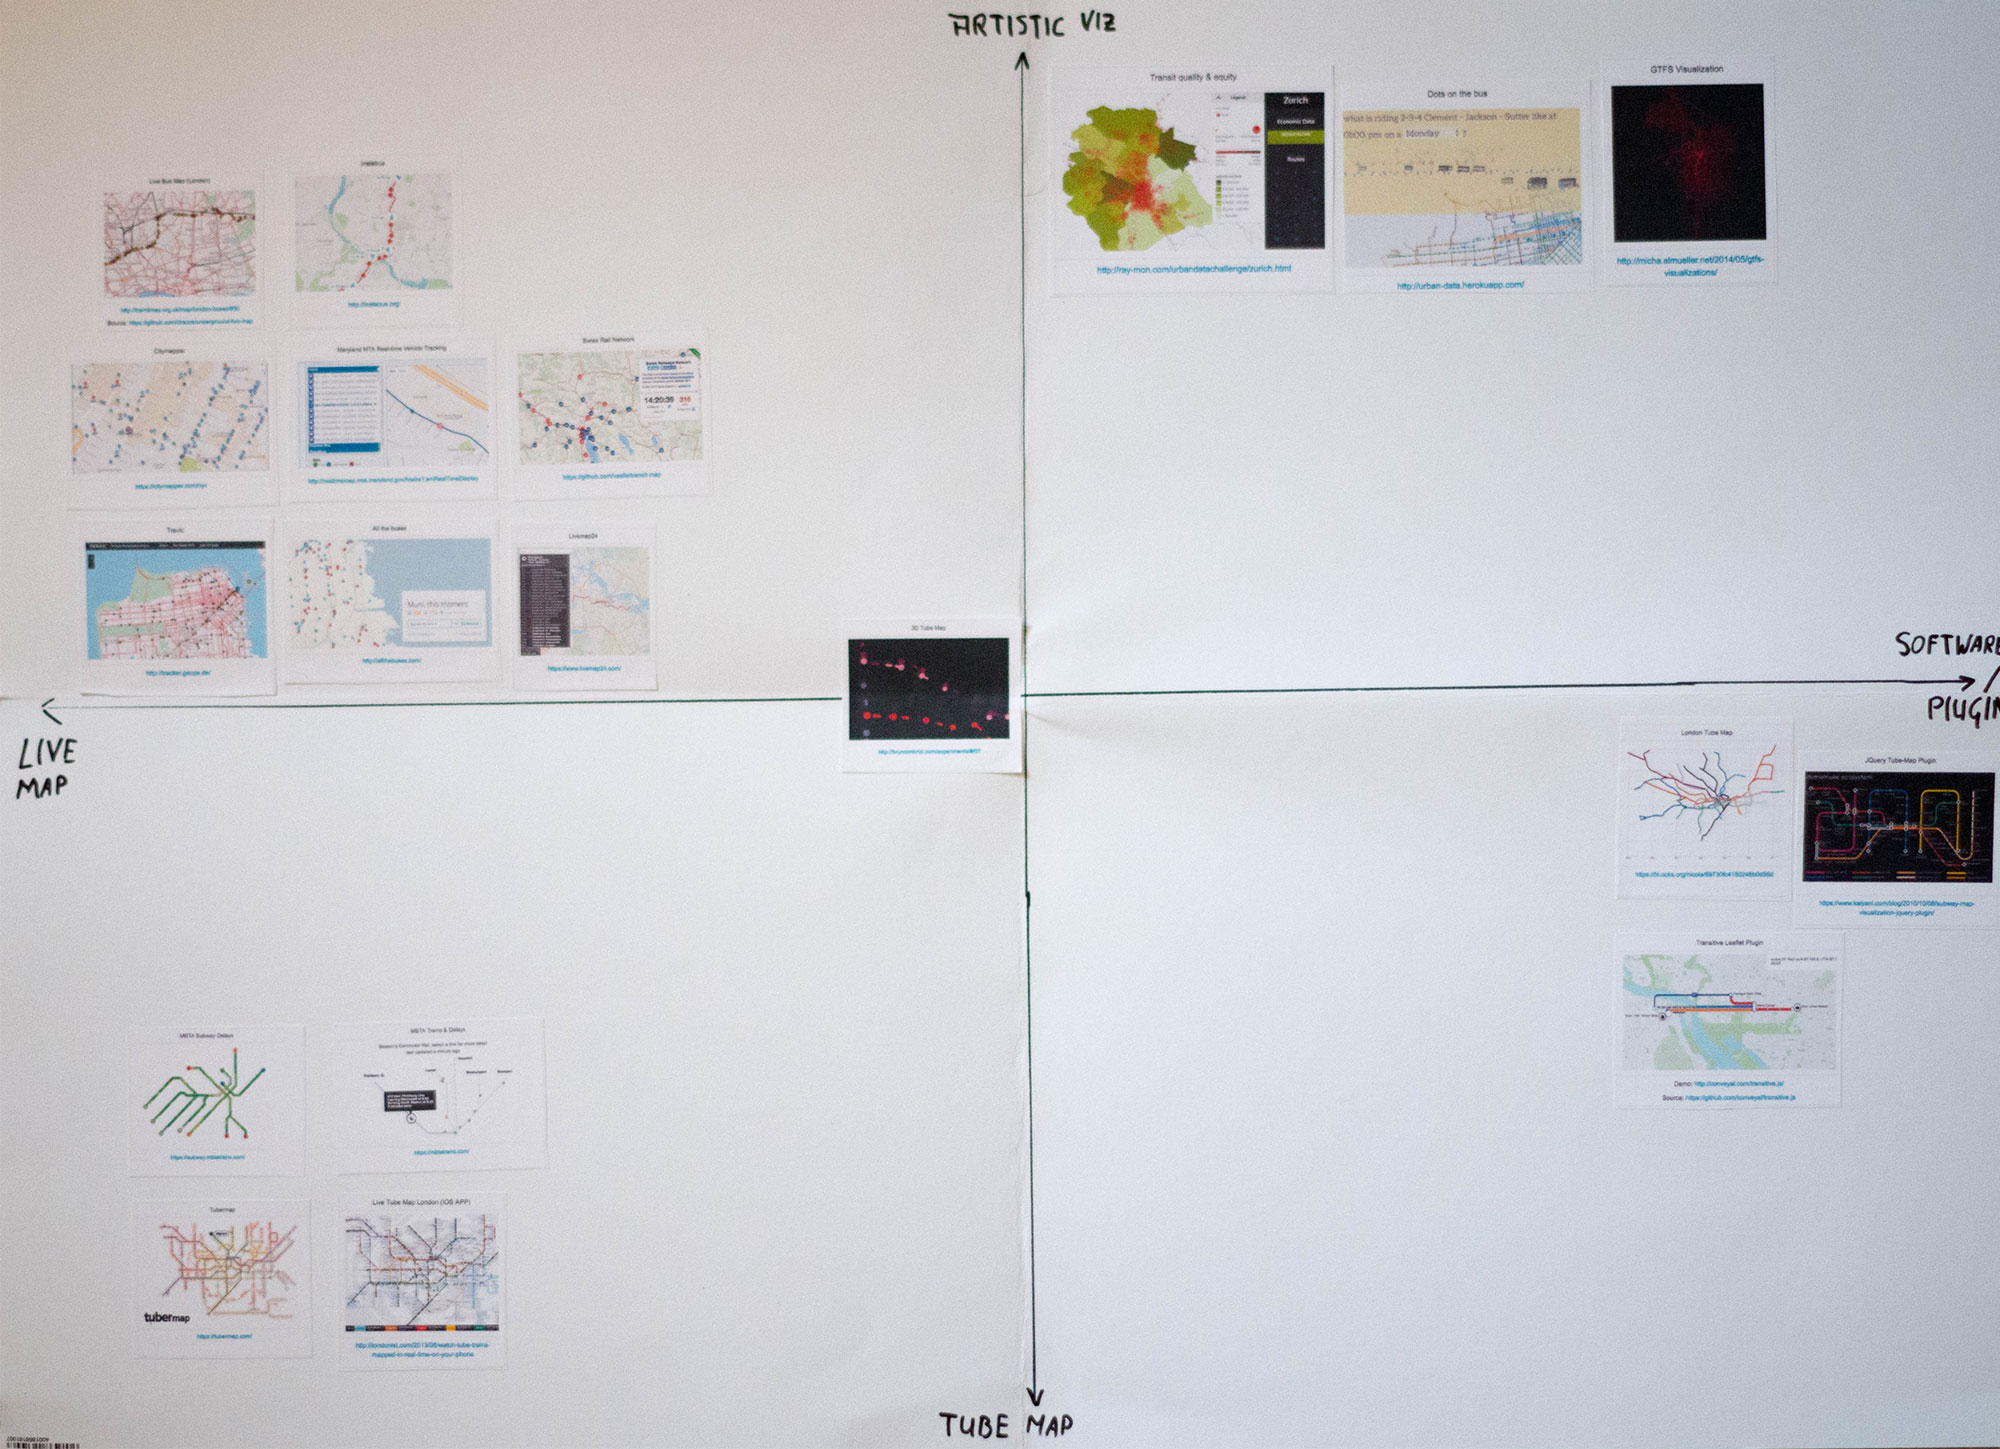
\includegraphics[width=0.5\textwidth]{2x2_matrix}
          \caption{2x2 Matrik Methode auf DIN A2}
          \label{fig:2x2_matrix}
        \end{center}
      \end{figure}

      Durch diese Ansicht wurde die Erkenntnis gewonnen, dass es schon viele Live Visualisierungen auf interaktiven Karten gibt, aber nur sehr wenig so genannten Tube-Maps. Auch sind bereits verschiedenste Tools zum generieren von GTFS basierten Visualisierungen vorhanden. Eine sehr ausführliche, aber bei weitem nicht vollständige, Liste über das Thema "Transit" wurde auf Github von der Community zusammengetragen \url{https://github.com/luqmaan/awesome-transit}. 

    % subsection discover (end)

    \subsection{Define}
    \label{sub:define}
      Aus der \texttt{Discover}-Phase sind verschiedene Ideen entstanden. Zum Beispiel sah eine Idee vor, die interaktive Karte mit anderen Visualisierungsformen zu kombinieren. So könnten die einzelnen Trips auch als Balkendiagramm dargestellt werden. Diese könnten die zurückgelegte Strecke darstellen. Dabei war gedacht das man zwischen diesen verschiedenen Visualisierungsformen hin- und herschalten kann. Auch der Ansatz dies mit einer Tube-Map zu verbinden wurde als Idee notiert und war Zeitweise als mögliches Ziel definiert. Aufgrund des Umfangs und der kurzen Zeitspanne einer Master-Thesis, konnte diese Richtung allerdings nicht näher verfolgt werden. Der Fokus sollte auf die Erstellung eines Prototypen oder Demonstrator für verschiedene neue Visualisierungsansätze von Vehicle Positionen liegen. Dabei war es wichtig, die GTFS-Daten zu visualisieren um sie gleichzeitig auch besser zu verstehen und die Zusammenhänge der GTFS-Spezifikation tiefer zu begreifen. Diese zwei Phasen des ersten Diamanten, nahmen ungefähr 6 Wochen Zeit in Anspruch.

      % TODO: Define better? Still a bit vague
      
    % subsection define (end)

    \subsection{Develop}
    \label{sub:develop}
      Zu beginn stellte sich die Frage, wie sich in kleinen Schritten an das komplexe Thema einer Live Visualisierung rangetastet werden kann. Die erste Hürde die zu nehmen ist, stellt die Animation vor nur \textbf{einem} Vehicle entlang der Polyline dar.
      Um eine Datengrundlage zu haben wurde ein möglichst vollständiges GTFS-Feed aus \texttt{TransitFeeds.com} ausgewählt und in die Datenbank importiert. Die Wahl fiel dabei auf das Boston-MBTA Feed. Die Herausforderung bestand nun darin, erste Daten aus der Datenbank an den Client zu senden und sie dort darzustellen. Dafür wurde versucht eine möglichst einfache Datenbankabfrage zu finden. Fast trivial ist das abfragen der Polyline: \colorbox{lightGrey}{\texttt{\color{white}{{\color{materialBlue} SELECT} * {\color{materialBlue}FROM} gtfs\_shapes {\color{materialBlue}WHERE} shape\_id = {\color{materialRed}12345}}}}
      Diese Daten werden als GeoJSON übertragen und lassen sich mit Mapbox-gl-js sehr einfach anzeigen. In der Karte ergibt sich daraus eine Route auf der sich ein Vehicle entlangbewegen kann.

      \begin{figure}[htbp]
        \begin{center}
          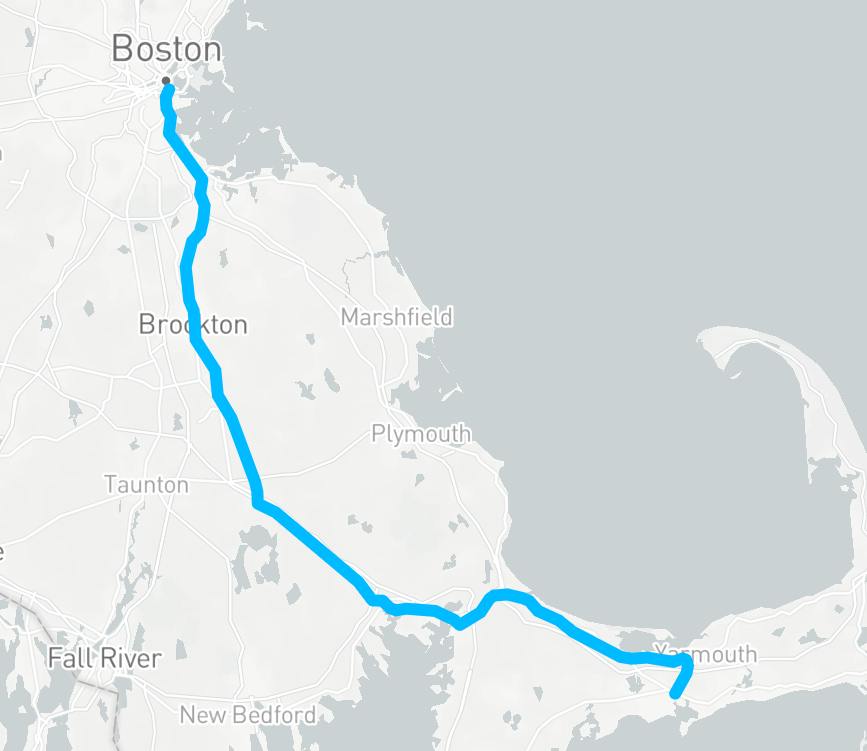
\includegraphics[width=0.5\textwidth]{prozess/draw_single_shape}
          \caption{Anzeigen einer einzigen Polyline in Boston}
          \label{fig:prozess/draw_single_shape}
        \end{center}
      \end{figure}
      
      Abbildung \ref{fig:prozess/draw_single_shape} zeigt das Ergebnis dieser ersten Iteration. Zu sehen ist bereits die Karte und eine blaue Polyline. Nachdem dieser Datensatz auf Client-Seite verarbeitet werden kann, musste das Backend wieder neue Abfragen von Daten ermöglichen. Dieser ständige Wechsel zwischen der Arbeit an Frontend und Backend zog sich durch das gesamte Projekt hinweg durch und stellte sich als sehr effektiv heraus. Erst durch die Arbeit am Frontend, wurde immer wieder klar, welche Daten überhaupt gebraucht und in welchem Format diese am besten sein müssen.\\

      Nachdem die Polyline auf die Karte gebracht wurde, machte es Sinn auch die einzelnen Stationen darzustellen. Damit die Daten besser verständlich sind und schnell auf ihren Inhalt untersucht werden können, öffnet sich beim anklicken ein Popup.

      \begin{figure}[htbp]
        \begin{center}
          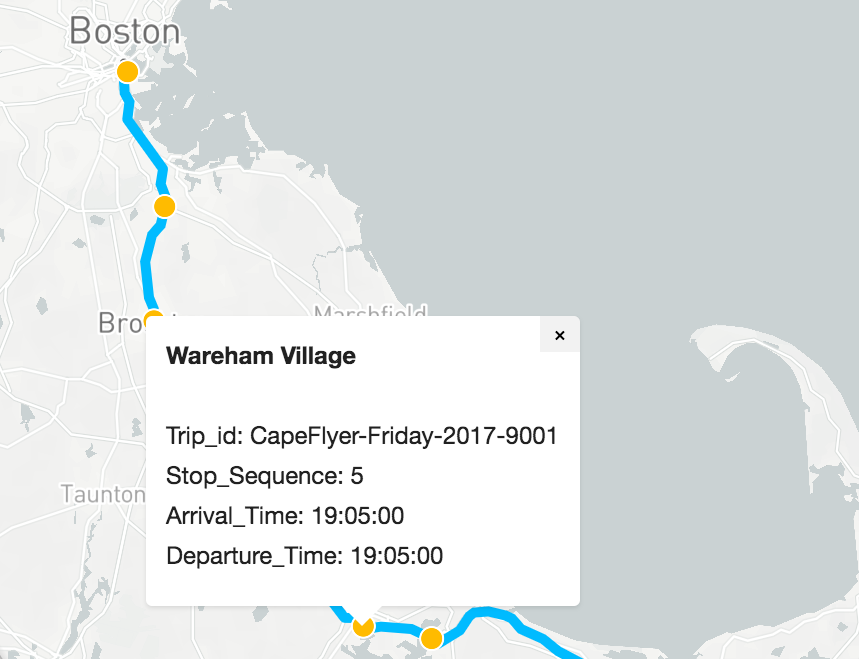
\includegraphics[width=0.5\textwidth]{prozess/add_stations}
          \caption{Hinzufügen von Stationen entlang der Polyline}
          \label{fig:prozess/add_stations}
        \end{center}
      \end{figure}

      An dieser Stelle sind bereits alle Informationen vorhanden, die benötigt werden um ein Vehicle zwischen den einzelnen Stationen fahren zu lassen. Ein Ansatz dafür, ist die Verwendung der Funktion \texttt{turf.along()}. Diese Funktion nimmt eine Polyline und gibt einen Punkt in einer bestimmten Entfernung entlang dieser Polyline zurück. Die Polyline ist bekannt, es fehlt die Distanz zwischen den einzelnen Stationen. Diese wird wie in Sektion \textit{\ref{ssub:station_matching} \nameref{ssub:station_matching}} im Backend berechnet. Des weiteren brauchen wir die Geschwindigkeit des Vehicles. Sind all diese Parameter vorhanden, lässt sich die Distanz des Vehicles (zwischen den einzelnen Stationen) zu jedem Zeitpunkt $t_i$ interpolieren.

      \begin{figure}[htbp]
        \begin{center}
          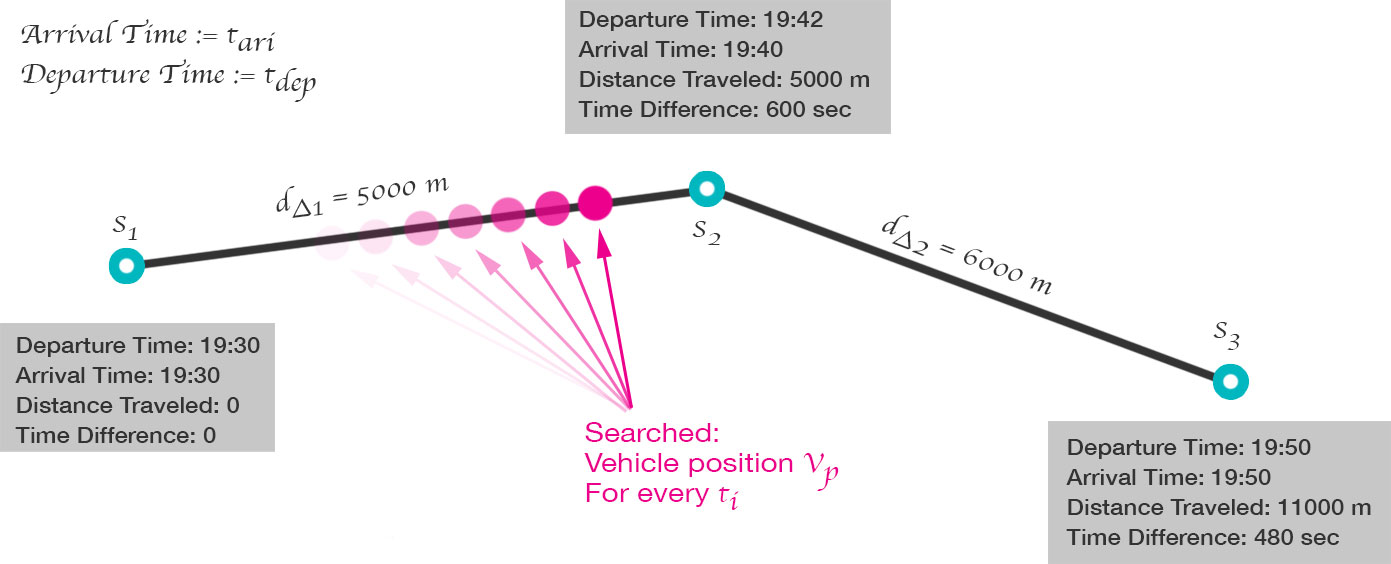
\includegraphics[width=0.9\textwidth]{interpolating_vehicle}
          \caption{Interpolation der Vehicle Position: $V_p$}
          \label{fig:interpolating_vehicle}
        \end{center}
      \end{figure}

      Die durchschnittliche Geschwindigkeit, die das Vehicle zwischen zwei Stationen hat, lässt sich über $v = \frac{d_\triangle}{TimeDifference}$ berechnen. Damit ist die Geschwindigkeit vorhanden und die interpolierte Distanz des Vehicles zu jedem Zeitpunkt $t_i$ lässt sich über die Formel der gleichförmigen Bewegung: $s_{neu} = v * t + s_0$ berechnen. Das resultierende $s_{neu}$ der Formel, kann dann an \texttt{turf.along(polyline, $s_{neu}$)} übergeben werden und gibt uns eine neue Position des Vehicles auf der Polyline zurück. Wird nun die Karte mit der neuen Position aktualisiert, fährt das Vehicle von Station zu Station. Natürlich müssen hier verschiedene Randbedingungen beachtet werden, beispielsweise was passiert, wenn das Vehicle am Ende angelangt ist oder wie werden Aufenthalte an einer Station beachtet.
      
      
      
    % subsection develop (end)


    \subsection{Deliver}
    \label{sub:deliver}
      
    % subsection deliver (end)
  % \begin{itemize}
  %   \item Überblick verschaffen
  %   \item Recherche Phase -> related visualizations
  %   \item What is not done?
  %   \item Limiting own scope
  % \end{itemize}

  % \begin{itemize}
  %   \item Introduce step by step solutions
  %   \item Screenshots
  %   \item Mockups
  %   \item Solving problems by iterative process
  % \end{itemize}
    
  % section problemlösungsprozess (end)
\end{newpage}